\documentclass[aspectratio=43, 10pt]{beamer}
\usepackage{tutorialSlide}
\usepackage{graphicx}               % Necessary to use \scalebox
\usepackage[absolute,overlay]{textpos}
\usepackage[normalem]{ulem}
\usepackage[makeroom]{cancel}
\renewcommand{\CancelColor}{\color{red}}
\newcommand{\curl}{{\textbf{curl}}}


\mode<presentation> {
\usetheme{AnnArbor}
\usecolortheme{dolphin}

% Configure and Customize the theme
%\setbeamertemplate{theorems}[numbered]
\setbeamercolor{alerted text}{fg=red}
% Change color scheme for blocks
\setbeamercolor*{block title example}{fg = ao(english), bg= antiquewhite}
\setbeamercolor*{block title}{fg = pigment, bg= blue!5}
\setbeamercolor*{block title alerted}{fg = red, bg= red!5}
}

\makeatletter
\newcommand\mysphere{%
  \parbox[t]{8pt}{\raisebox{0.2pt}{\beamer@usesphere{item projected}{bigsphere}}}}
\makeatother




%***************************************************************************
%***************************************************************************
\begin{document}
\title{A Concise (though Heuristic) Derivation of AMP}
\author{Weijia Zheng 
\thanks{I mainly took reference to: "A Simple Derivation of AMP and its State Evolution via First-Order Cancellation" by P. Schniter. This is a very readable file on this topic.}
}

\institute[IE@CUHK] % Your institution as it will appear on the bottom of every slide, may be shorthand to save space
{
\textit{Department of Information Engineering} \\ % Your institution for the title page
\textit{The Chinese University of Hong Kong} \\
\medskip
wjzheng@link.cuhk.edu.hk % Your email address
}
\date{May 15, 2025}

\setcounter{framenumber}{-1}
\frame{\titlepage}
%***************************************************************************
%***************************************************************************




\begin{frame}
\frametitle{Overview} % Table of contents slide, comment this block out to remove it
\tableofcontents % Throughout your presentation, if you choose to use \section{} and \subsection{} commands, these will automatically be printed on this slide as an overview of your presentation
\end{frame}



\AtBeginSection[]
  {
     \begin{frame}<beamer>
     \frametitle{Overview}
     \tableofcontents[currentsection]
     \end{frame}
  }
  
% Section 1: Introduction
\section{Introduction}
\begin{frame}{High dimensional linear regression problem}
    \vspace{-3mm}
    \begin{block}{Liner regression formulation}
        Consider a problem of the form $\bold{y} = \bold{A} \boldsymbol{\beta}_0 + \bold{w}.$ We want to reconstruct $\boldsymbol{\beta}_0$ from $\bold{y}$. 
    \end{block}

    \vspace{-2mm}
    \begin{figure}
        \centering
        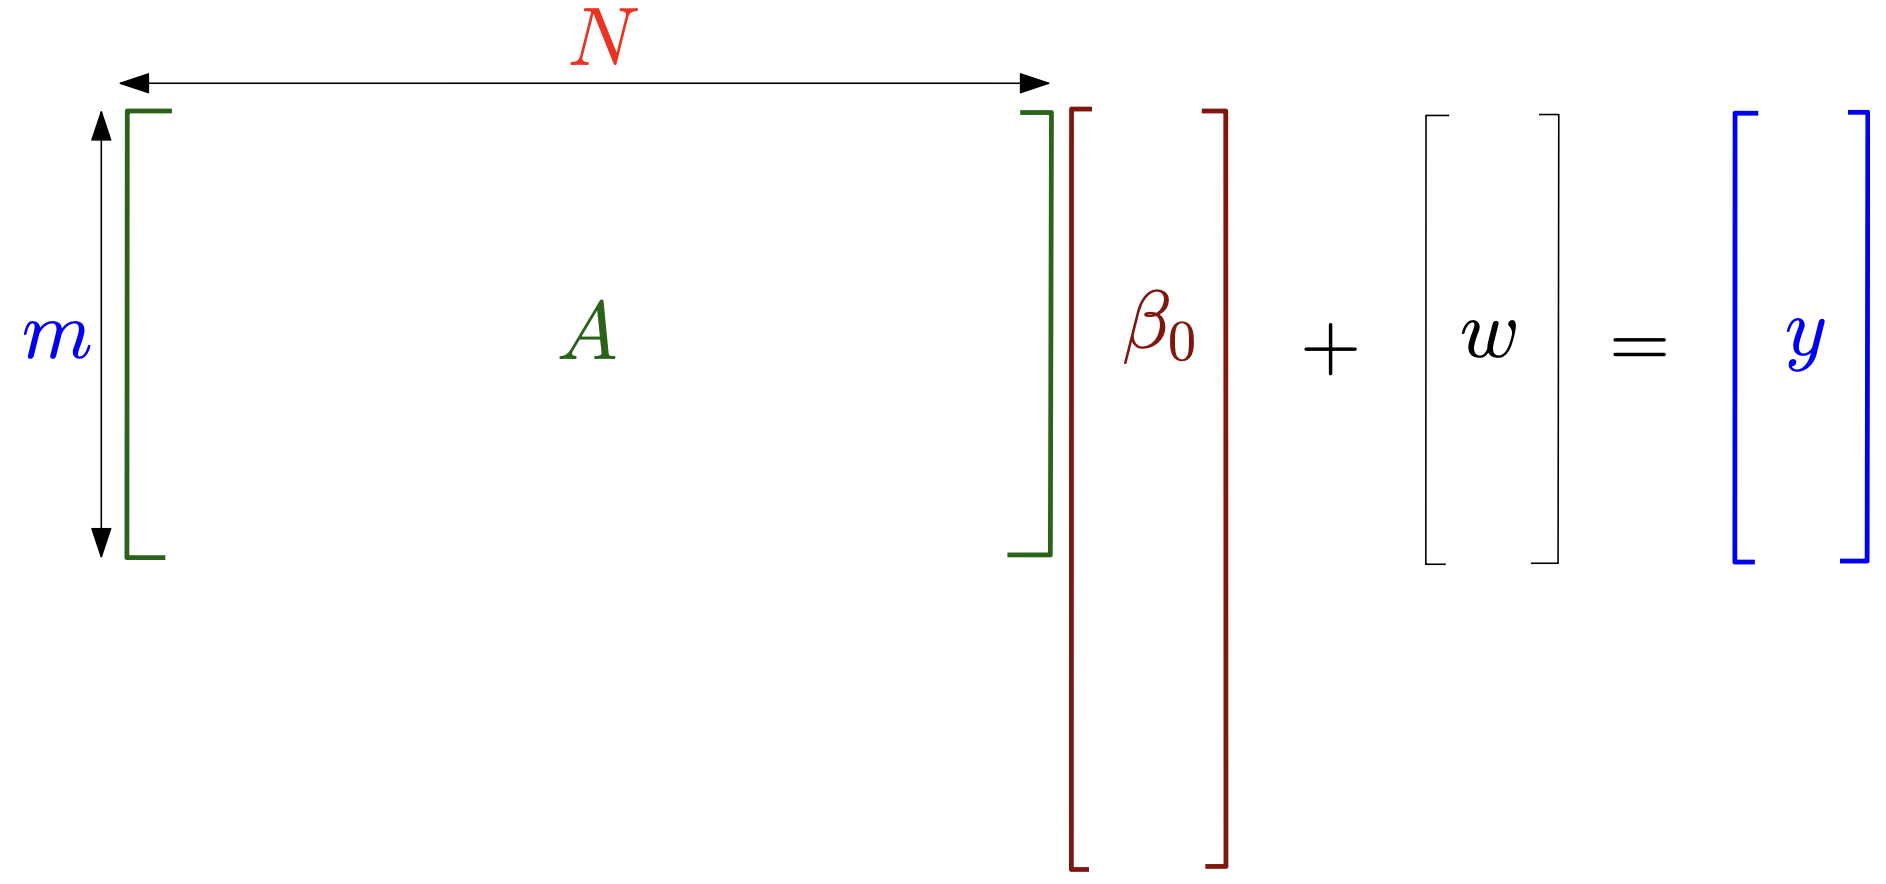
\includegraphics[width=0.6\linewidth]{figures/vis_formulation.png}\footnote{Figure copied from "Approximate Message Passing for Statistical Inference and Estimation" (good lecture slides with Youtube video recording)}
    \end{figure}

    \pause
    \vspace{-4mm}
    \begin{itemize}
        \item $\bold{y}$: an observed length-$m$ measurement vector
        \item $\bold{w}$: an unknown length-$m$ noise. Assume $w \sim_{iid} \mathcal{N}(0, \tau_w)$
        \item $\bold{A}$: a known big $m\times N$ (normalized) matrix with $m<N$, $\frac{m}{N} \to \delta \in \Omega(1)$ 
        \item $\boldsymbol{\beta}_0$: a length-$N$ signal vector to find
    \end{itemize}
\end{frame}

\begin{frame}
    \vspace{-0.3cm}
    \begin{figure}
            \centering
        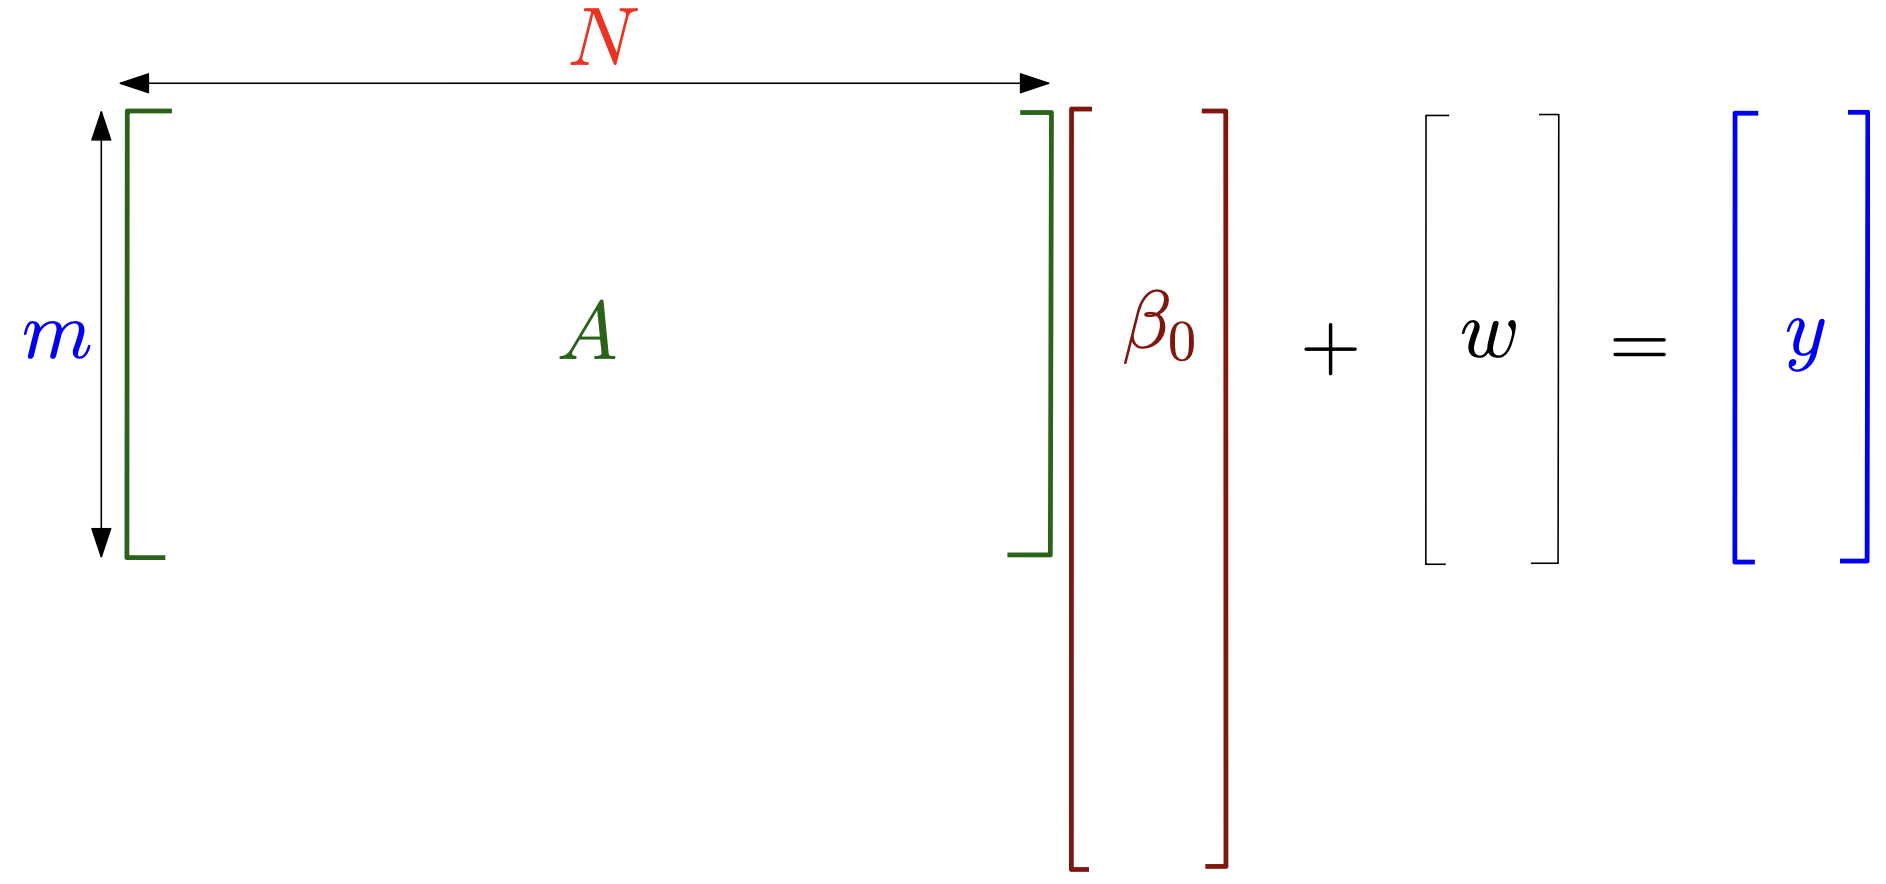
\includegraphics[width=0.7\linewidth]{figures/vis_formulation.png}
    \end{figure}

    \vspace{-0.2cm}
    \begin{block}{Prior knowledge on $\boldsymbol{\beta}_0$: sparsity}
        People may assume sparsity of $\boldsymbol{\beta}_0$. That is, it has only $K\ll N$ nonzero entries. 
    \end{block}

    \pause
    \begin{block}{NP-hardness of sparse recovery in general}
        Assume $K$-sparse, the problem: for any given $\bold{A}$, find $\arg\min_{\boldsymbol{\beta}} \| \bold{A}\boldsymbol{\beta} - \bold{y}  \|^2$ is NP-hard. In fact, even if we know the entries' values of the ground-truth $\boldsymbol{\beta}_0$, the problem is still NP-hard. \footnote{For the NP-hardness: one can do reduction using  Exact Cover by 3-Sets (X3C).}
    \end{block}
    
\end{frame}

\begin{frame}{(Sparsity inspired) LASSO}
    \vspace{-4mm}
    \begin{columns}
        \begin{column}{0.66\textwidth}
            \begin{block}{LASSO and ISTA}
            $$\min_{\boldsymbol{\beta}} \underbrace{\frac{1}{2}\| \bold{y} - \bold{A} \boldsymbol{\beta} \|^2}_{\triangleq g(\boldsymbol{\beta})} + \lambda \| \boldsymbol{\beta} \|_1. \notag$$
    
        Iterative Soft-Thresholding Algorithm (ISTA) can solve this: 
            \begin{align}
                \bold{v} &= \bold{y} - \bold{A} \boldsymbol{\beta}^t \notag \\ 
                \boldsymbol{\beta}^{t+1} &= \texttt{soft}(\boldsymbol{\beta}^{t}+s\bold{A}^T \boldsymbol{v}^{t}; s\lambda). \notag 
            \end{align}
            Writing it into a more intuitive form: 
            \begin{equation}
                \boldsymbol{\beta}^{t+1} = \underbrace{\texttt{soft}( \underbrace{\boldsymbol{\beta}^{t} - s\nabla g(\boldsymbol{\beta^{t}})}_{\text{grad. descent}}; s\lambda)}_{\text{impose sparsity}}. \notag
            \end{equation}
            \end{block}
        \end{column}
        
        \begin{column}{0.3\textwidth}
            $$\nabla g(\boldsymbol{\beta}) = \bold{A}^T (\bold{A} \boldsymbol{\beta} - \bold{y}).$$

            \vspace{-3mm}
            \begin{figure}
                \centering
                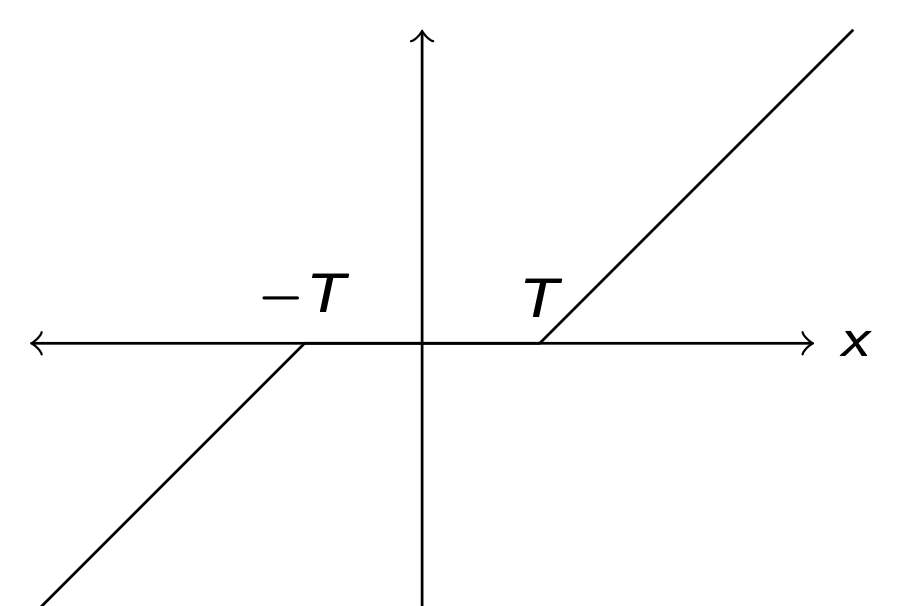
\includegraphics[width=0.9\linewidth]{figures/ST_function.png}
                \caption{$\texttt{soft}(x,T)$.}
            \end{figure}

            \vspace{-3mm}
            One can tune the parameter $\lambda$ to control the sparsity, and $s$ here works as a stepsize. 

            \vspace{3mm}
            LASSO is convex in $\boldsymbol{\beta}$.
        \end{column}
    \end{columns}
\end{frame}

\begin{frame}{AMP Framework}
    \vspace{-3mm}
    \begin{block}{LASSO \& ISTA are great, but...}
        LASSO is motivated by \textbf{sparsity} alone, and it does not consider the signal's prior distribution, which may sometimes be available. Thus, people want to integrate the knowledge of $\boldsymbol{\beta}_0 \sim_{iid} p_{\beta}$ into inference of $\boldsymbol{\beta}_0$.\footnote{AMP does not explicitly assume sparsity of $\boldsymbol{\beta}_0$.} 
    \end{block}

    The problem then changes to find an $\hat{\boldsymbol{\beta}}$ for $\bold{y}= \bold{A} \boldsymbol{\beta}_0 + \bold{w}, ~~ \text{while } \boldsymbol{\beta}_0 \sim_{iid} p_{\beta}$. 


    \pause
    \vspace{0.2cm}
    We compare the procedure of AMP and ISTA at below. 

    \begin{columns}
        \begin{column}{0.5\textwidth}
            \begin{block}{Approximate message passing (AMP)}
                \vspace{-5mm}
                \begin{align}
                    \bold{v}^{t} &= \bold{y} - \bold{A} \boldsymbol{\beta}^t + \underbrace{\frac{\boldsymbol{v}^{t-1}}{m} \sum_{j=1}^N \eta_{t-1}'(r_j^{t-1})}_{\textcolor{red}{\text{Onsager correction term}}} \notag \\ 
                    \boldsymbol{\beta}^{t+1} &= \eta_t( \underbrace{\boldsymbol{\beta}^{t}+s\bold{A}^T \bold{v}^{t}}_{\triangleq \boldsymbol{r}^{t}} ). \notag 
                \end{align}
            \end{block}
        \end{column}

        \begin{column}{0.45\textwidth}
            \vspace{-13mm}
            \begin{block}{Iterative Soft Thresholding Algo. (ISTA)}
                \vspace{-5mm}
                \begin{align}
                    \bold{v}^{t} &= \bold{y} - \bold{A} \boldsymbol{\beta}^t \notag \\ 
                    \boldsymbol{\beta}^{t+1} &= \texttt{soft}(\boldsymbol{\beta}^{t}+s\bold{A}^T \bold{v}^{t}; s\lambda). \notag 
                \end{align}
            \end{block} 
            
        \end{column}
    \end{columns}
\end{frame}

\begin{frame}
    There are some requirements in $\boldsymbol{A}$, the sensing/measurement matrix. In general, assume $\boldsymbol{A}$ to be entry-wisely iid generated with $\mathbb{E} a_{ij}=0$ and $\mathbb{E} (a_{ij}^2) = \frac{1}{m}$ suffices.

    \vspace{3mm}
    In fact, in the paper we will go through, \textcolor{red}{they assume $a_{ij} \in \mathcal{U} \{ \pm \frac{1}{\sqrt{m}}\}$}. But this is mainly to simplify the proof, and it can be extended to more general cases. 

    \pause
    
    \begin{block}{AMP iteration}
        \begin{columns}
            \begin{column}{0.5\textwidth}
                \begin{align}
                    &\bold{v}^{t} = \bold{y} - \bold{A} \boldsymbol{\beta}^t + \underbrace{\frac{\boldsymbol{v}^{t-1}}{m} \sum_{j=1}^N \eta_{t-1}'(r_j^{t-1})}_{\textcolor{red}{\text{Onsager correction term}}} \notag \\ 
                    & \boldsymbol{\beta}^{t+1} = \eta_t( \underbrace{\boldsymbol{\beta}^{t}+s\bold{A}^T \bold{v}^{t}}_{\triangleq \boldsymbol{r}^{t}} ). \notag 
                \end{align}
            \end{column}
    
            \hspace{-5mm}
            \begin{column}{0.6\textwidth}
                \begin{itemize}
                    \item $\boldsymbol{r}^t \in \mathbb{R}^{N}$, termed \textbf{"effective observation"}
                    \item $\eta_t(\cdot)$ is called a "denoising function" $[\eta_t(\boldsymbol{r})]_j = \eta_t(r_j)$ 
                    \item \textcolor{brown}{In ISTA, $\eta_t =\texttt{soft}()$ and we do not consider any correction term}
                \end{itemize}
            \end{column}
        \end{columns}
    \end{block}
    
    \begin{block}{Main purpose of the paper}
        Simply to understand: why there is such an "Onsager term", and what should be chosen as the denoising function $\eta_t(\cdot)$. 
    \end{block}
\end{frame}


\section{Onsager Correction Derivation}
\begin{frame}{Why the Onsager Correction?}
    \vspace{-5mm}
    \begin{block}{AMP Iteration Recap}
        For \(\bold{y} = \bold{A} \boldsymbol{\beta}_0 + \bold{w}\), AMP iterates:
        \begin{align*}
            \bold{v}^{t} &= \bold{y} - \bold{A} \boldsymbol{\beta}^t + \underbrace{\frac{\bold{v}^{t-1}}{m} \sum_{j=1}^N \eta_{t-1}'(r_j^{t-1})}_{\textcolor{red}{\text{Onsager correction term}}}, \\
            \boldsymbol{\beta}^{t+1} &= \eta_t \left( \boldsymbol{\beta}^t + \bold{A}^T \bold{v}^t \right) \triangleq \eta_t(\bold{r}^t).
        \end{align*}
    \end{block}

    \pause
    \begin{itemize}
        \item Partial goal: Ensure \(\bold{r}^t - \boldsymbol{\beta}_0 \approx  \text{Gaussian noise}\). (See next page.)
        \item \textcolor{brown}{Onsager term adjusts \(\bold{v}^t\) to cancel error correlations.}
    \end{itemize}
    
    \begin{block}{Our focus soon}
        Derive the Onsager term by analyzing the difference between the effective observation and ground-truth signal \(\bold{e}^t = \bold{r}^t - \boldsymbol{\beta}_0\).
    \end{block}
\end{frame}

\begin{frame}{Correction terms work}


Correction terms push the effective observation to $\boldsymbol{\beta}_0 + $ some (tiny) Gaussian. 

\vspace{2mm}
Comparing with vanilla IST, such effect is decisive.  

\begin{figure}
    \centering
    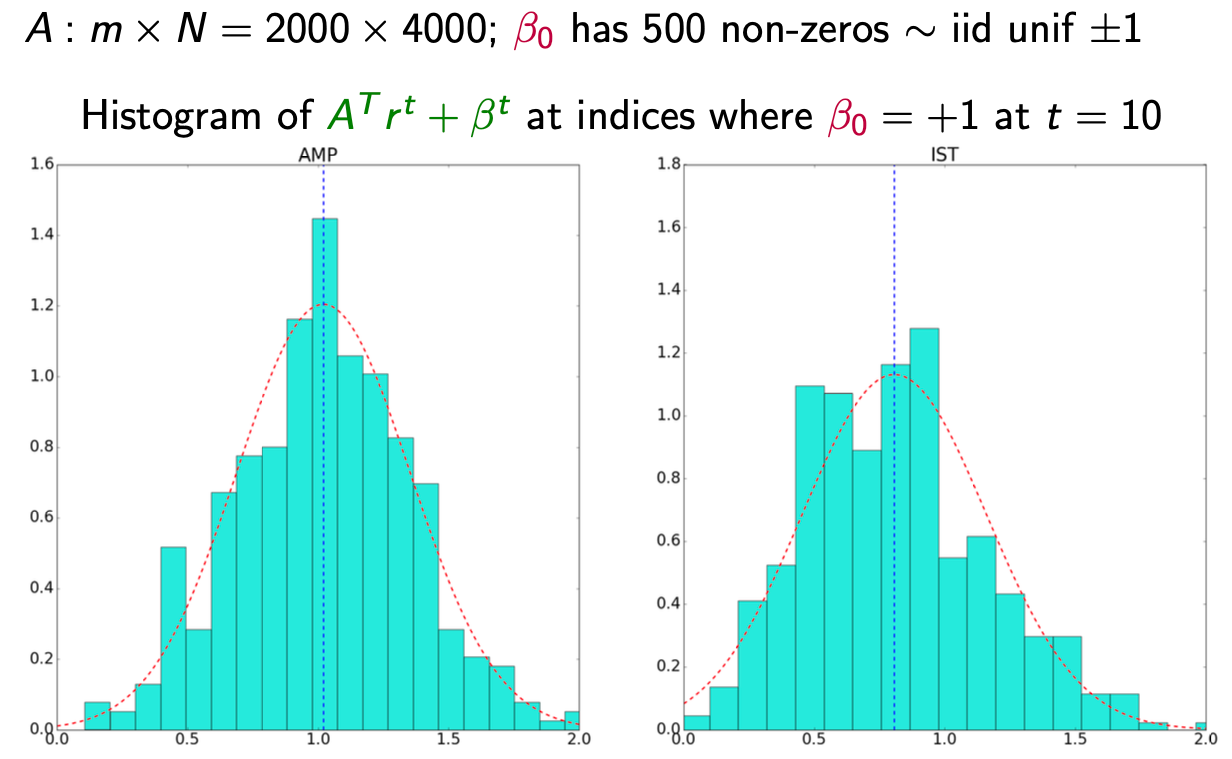
\includegraphics[width=0.84\linewidth]{figures/AMPvsISTA.png}
    % \caption{Caption}
    \label{fig: amp vs. ist}
\end{figure}

    
\end{frame}

\begin{frame}{Error Analysis}
    % \small 
    \vspace{-2mm}
    \begin{block}{Define the Error}
        Recall \(\bold{r}^t = \boldsymbol{\beta}^t + \bold{A}^T \bold{v}^t\). The error is: $\bold{e}^t = \bold{r}^t - \boldsymbol{\beta}_0 = \left( \boldsymbol{\beta}^t + \bold{A}^T \bold{v}^t \right) - \boldsymbol{\beta}_0.$
        
        Substitute \(\bold{v}^t = \bold{y} - \bold{A} \boldsymbol{\beta}^t + \bold{u}^t\), where $\bold{u}^t$ denotes (any) correction term:
        \[
        \bold{r}^t = \boldsymbol{\beta}^t + \bold{A}^T \left( \bold{y} - \bold{A} \boldsymbol{\beta}^t + \bold{u}^t \right).
        \]

        Since \(\bold{y} = \bold{A} \boldsymbol{\beta}_0 + \bold{w}\), $\bold{A}^T \bold{y} = \bold{A}^T (\bold{A} \boldsymbol{\beta}_0 + \bold{w}).$
        Then 
        \begin{equation}
            \boldsymbol{e}^t = (\boldsymbol{I}-\boldsymbol{A}^T \boldsymbol{A})(\boldsymbol{\beta}^t - \boldsymbol{\beta}_0) + \boldsymbol{A}^T (\boldsymbol{w}+ \boldsymbol{u}^t) \notag. 
        \end{equation}
    \end{block}

    \pause 
    
    \vspace{-2mm}
    \begin{block}{Zooming in the $l$-th entry}
        We focus more on $\boldsymbol{\beta}^t$. $\boldsymbol{\beta}^t=\eta_{t-1}(\boldsymbol{r}^{t-1})$. Its $l$-th entry is $\beta^t_l = \eta_{t-1}(r^{t-1}_l)$. 

        And we decompose $r_l^{t-1}$ as: 
        \begin{equation}
            r_l^{t-1} = \beta_l^{t-1} + \sum_{k}a_{kl}v_k^{t-1} = 
            \underbrace{\beta_l^{t-1} + \sum_{k\neq i}a_{kl}v_k^{t-1}}_{\triangleq r_{l \setminus i }^{t-1}, ~\text{assumed indep. of $\{a_{ij}\}_j$}} + a_{il}v_i^{t-1}. 
        \end{equation}
    \end{block}
\end{frame}

% \begin{frame}{Independence Lemma}
% \begin{lemma}
%     Consider a quantity $\gamma_i = \sum_{j=1}^N a_{ij} z_j$, where $a_{ij}$ are realizations of iid random variables with zero mean and variance $=\frac{1}{m}$. If ${a_{ij}}$ are drawn independently from $\{z_j\}$, 
% \end{lemma}
% \end{frame}

\begin{frame}
    \vspace{-3mm}
        \begin{block}{Error decomposition}
        Then the error (its $j$-th entry) becomes  
        \begin{align}
             e_j^t = & \sum_i a_{ij} \left[ \sum_{l \neq j} a_{il} (\beta_{0,l} - \textcolor{brown}{\beta_l^t}) + w_i + u_i^t \right] \notag \\
            = & \underbrace{\sum_{i}a_{ij} \sum_{l \neq j} a_{il} [\beta_{0,l}-\textcolor{teal}{\eta_{t-1}(r_{l \setminus i}^{t-1})}] + \sum_{i}a_{ij}w_{i}}_{\text{Indepndence + CLT} \implies \sim_d \text{ Gaussian} } \notag  \\ 
            & + \underbrace{\sum_{i}a_{ij} \left[ u_i^{t} 
            +\sum_{l \neq j} \textcolor{blue}{-\frac{v_i^{t-1}}{m}\eta_{t-1}'(r_{l\setminus i}^{t-1})} \right]}_{\triangleq T_1\text{ ,want to make it small when~} m \text{ is large}} \notag \text{   ~~$a_{ij}$ and $v_i^{t-1}$ are coupled!}
        \end{align}
    
        In the above, we used Taylor expansion: 
        $$\textcolor{brown}{\beta_l^t}=\eta_{t-1}(r_l^{t-1}) = \eta_{t-1}(r_{l\setminus i}^{t-1} + a_{il} v_i^{t-1})\approx 
        \textcolor{teal}{\eta_{t-1}(r_{l\setminus i}^{t-1} )} +
        \textcolor{blue}{a_{il}v_i^{t-1} \eta_{t-1}'(r_{l\setminus i}^{t-1})}.
        $$
        And, we used $a_{il}^2 = \frac{1}{m}$. 
        \end{block}
\end{frame}

\begin{frame}
    \vspace{-1mm}
    \small 
    \begin{block}{Focus on Correction Term}
        The last error term (the not Gaussian one) is the only term involving \(\bold{u}^t\):
        \begin{equation}
            T_1 = \sum_{i}a_{ij} \left[ u_i^{t} 
            -\sum_{l \neq j}\frac{v_i^{t-1}}{m}\eta_{t-1}'(r_{l\setminus i}^{t-1}) \right] 
            \label{error}
        \end{equation}

        Note that \(\bold{u}^t\) is some correction term free to choose. And we wish such choice to make $T_1$ small. 

        We can see why Onsager is good by observing its form: $u_i^t \triangleq  \frac{v_i^{t-1}}{m} \sum_{l=1}^N \eta_{t-1}'(r_l^{t-1}). $

        We can proceed an estimation of $T_1$: 
        \begin{align}
            T_1 &\approx_{\text{2 order Taylor}} \approx \sum_{i}a_{ij} \left[ \frac{v_i^{t-1}}{m} \sum_{l=1}^N \eta_{t-1}'(r_l^{t-1})  - \sum_{l \neq j}\frac{v_i^{t-1}}{m}\eta_{t-1}'(r_{l\setminus i}^{t-1})\right] \\
            & \approx \frac{1}{m}\sum_{i}a_{ij} v_i^{t-1} \left[ \eta_{t-1}'(r_j^{t-1}) +   \sum_{l\neq j} a_{il} v_i^{t-1} \eta_{t-1}''(r_{l \setminus i}^{t-1}) \right] \in \mathcal{O}(\frac{1}{\sqrt{m}})
            \label{error asymptotics}
        \end{align}  

        The two terms in eq. (\ref{error asymptotics}) are both $\mathcal{O}(\frac{1}{\sqrt{m}})$. And \textcolor{red}{it is hard to design a better correction term (without sacrificing too much computational complexity.})
    \end{block}
\end{frame}


\section{State Evolution}
\begin{frame}{Completing Error Estimation}
    \vspace{-0.3cm}
    \begin{block}{Recap: Error Decomposition}
        From the previous slide, the error \( e_j^t \) is:
        \begin{equation}
            e_j^t = & \underbrace{ \underbrace{\sum_{i}a_{ij} \sum_{l \neq j} a_{il} [\underbrace{\beta_{0,l}-\eta_{t-1}(r_{l \setminus i}^{t-1})}_{\triangleq \epsilon_{l \setminus i}^t}]}_{=S_1} + \underbrace{\sum_{i}a_{ij}w_{i}}_{=S_2}}_{\text{Indepndence + CLT} \implies \sim_d \text{ Gaussian} } +  \underbrace{\xcancel{T_1}}_{\text{ignored when } m \gg 1} \notag
        \end{equation}
    \end{block}

    $S_2$ is much easier to handle, it has zero mean and variance $= \tau_w$. ($\boldsymbol{w}$'s power)

    \vspace{0.2cm}

    $S_1$ has mean zero. And it has variance $\frac{1}{m^2}\sum_{i=1}^m \sum_{l\neq j} (\epsilon_{l \setminus i}^t)^2 \approx \frac{n}{m}\frac{1}{n}\sum_{l=1}^n (\epsilon_l^t)^2$, where $\epsilon_l^t \triangleq \beta_{0,l} - \eta_{t-1}(r_l^{t-1})$ is the \textcolor{red}{effective noise}. 

    \vspace{0.2cm}

    People denote $\mathcal{E}^t = \frac{1}{n} \sum_{l=1}^n (\epsilon_l^t)^2 $. Then one can write 
    \begin{equation}
        e_j^t = \beta_{0,j} - r_j^t \sim_{\text{approx.}} \mathcal{N}(0, \underbrace{\delta^{-1} \mathcal{E}^t + \underbrace{\tau_w}_{\text{fixed}}}_{\triangleq \tau_r^t}).  \notag
    \end{equation}
\end{frame}


\begin{frame}{State Evolution: Predicting Performance}
    \vspace{-2mm}
    \begin{block}{State Evolution Equations}
        Track error variance \( \tau_r^t = \text{Var}(r_j^t - \beta_{0,j}) \):
        \[
        \tau_r^t = \delta^{-1} \mathcal{E}^t + \tau_w, 
        \quad \mathcal{E}^{t+1} = \mathbb{E} \left[ \eta_t(\beta_{0} + Z_t) - \beta_{0} \right]^2, \quad Z_t \sim \mathcal{N}(0, \underbrace{\tau_r^t}_{\approx \frac{\| \boldsymbol{v}^t \|^2}{m}}).
        \]
    \end{block}
    
    \vspace{3mm}
    \begin{itemize}
        \item \( \mathcal{E}^t \): Mean squared error (MSE) of denoiser at iteration \( t \).
        \item It predicts AMP’s MSE without running the algorithm.
    \end{itemize}

    \vspace{5mm}
    Basically, $\mathcal{E}^t$ is what we can control in $\tau_r^t$. Hence we want to choose a function $\eta_t()$ to minimize it! 

    \vspace{5mm}
    Now, we see why people choose $\eta_t \gets $ posterior mean estimator (PME).\footnote{One can use Tweedie's formula here, when $\beta_0$'s prior is known.}
    
\end{frame}


%***************************************************************************
%***************************************************************************
\end{document}





































